\chapter{Frobenius自同构与类域论}\label{L2}
\lecturedate{2020/02/19}
\sourcepage{11}
我们已经描述了$\Q^{\mathrm{ab}}$和$\Gal(\Q^{\mathrm{ab}}/\Q)$。本讲研究任意代数数域$F$的阿贝尔扩张$L/F$。我们将利用类域论证明Kronecker--Weber定理，并介绍分类定理：阿贝尔扩张$L/F$可以由$F$的某些理想类群\znote{理想类群 $\mathrm{Cl}(F)=I_F/P_F$ 是分式理想群模去主分式理想群，其阶 $h_F$ 称为类数，数域的类数有限。它衡量 $\OO_F$ 偏离唯一分解的程度：$h_F=1$ 当且仅当 $\OO_F$ 是唯一分解整环；非平凡类群的存在正是类域论要处理的现象：例如 $\mathrm{Cl}(\Q)=1$，而 $\OO_{\Q(\sqrt{-5})}$ 的类数为 $2$，这对应 $2\cdot3=(1+\sqrt{-5})(1-\sqrt{-5})$ 给出的两种本质不同的分解。[来源：nLab "ideal class group"，\url{https://ncatlab.org/nlab/show/ideal+class+group}（Last revised 2018-05-11；2026-11-14 访问）。]}来参数化。
\section{代数数论预备知识}\label{L2S1}
按照定义，代数数域$F$是$\Q$的有限扩张。记$\OO_F$为$F$中的代数整数环\znote{$\OO_F$ 是 $F$ 的唯一极大序：任何由 $F$ 中代数整数构成的环都含于它。常见误解是把它当作唯一分解整环——$\OO_{\Q(\sqrt{-5})}=\Z[\sqrt{-5}]$ 中 $6=2\cdot3=(1+\sqrt{-5})(1-\sqrt{-5})$ 就是经典反例。它之所以仍是开展数论的良好舞台，是因为它是 Dedekind 整环：元素未必唯一分解，但理想一定唯一分解。[来源：Neukirch, \textit{Algebraic Number Theory}, Grundlehren der mathematischen Wissenschaften 322, 第 I 章 §8（本讲参考文献）。]}（换言之，$\OO_F$是$\Z$在$F$中的整闭包）。一般而言，$\OO_F$不是唯一分解整环，但它是Dedekind整环。设$L/F$为有限扩张，$D$为$\OO_F$在$L$中的整闭包。于是有以下性质。\idx{代数整数环}\idx{Dedekind整环}
\begin{property}
$D$是Dedekind整环，因此$D$中每个非零真理想都能唯一写成素理想的乘积。
\end{property}
\begin{definition*}{分歧指数与剩余次数}\idx{分歧指数}\idx{剩余次数}
$\OO_F$的每个非零素理想$\p$都满足$\p D\ne D$，因此有分解
\[\p D=\Pp_1^{e_1}\cdots\Pp_r^{e_r},\]
其中$\Pp_1,\ldots,\Pp_r$是$D$中满足$\Pp_j\cap\OO_F=\p$的素理想。$e_j$称为$\Pp_j$在$\p$上的\textbf{分歧指数}\znote{分歧指数 $e_j$ 是 $\p$ 在 $\Pp_j$ 中的重数，即 $e_j=v_{\Pp_j}(\p D)$，由 $\Pp_j^{e_j}\parallel\p D$ 刻画；它计量 $\p$ 在 $\Pp_j$ 处「重复」了多少次，$e_j>1$ 就是分歧的定量含义。易错之处在于：$e_j$ 依赖于 $\Pp_j$，同一 $\p$ 上方的不同素理想可以有不同分歧指数；但在 $L/F$ 为 Galois 时它们全都相等。[来源：Neukirch, \textit{Algebraic Number Theory}, Grundlehren der mathematischen Wissenschaften 322, 第 I 章 §8（本讲参考文献）。]}。
\sourcepage{12}
此外，$\OO_F/\p$与$D/\Pp_j$都是有限域\znote{$\OO_F/\p$ 称为 $\p$ 的\textbf{剩余域}（residue field），常记作 $\kappa(\p)$；$D/\Pp_j$ 是 $\Pp_j$ 的剩余域。二者都是有限域，而 $f_j=[\kappa(\Pp_j):\kappa(\p)]$ 是剩余域扩张的次数——这正是「剩余次数」一名的由来。剩余域之所以重要，是因为它与分歧指数 $e_j$ 一起完整刻画了 $\p$ 在 $\Pp_j$ 处的分解行为。[来源：Neukirch, \textit{Algebraic Number Theory}, Grundlehren der mathematischen Wissenschaften 322, 第 I 章 §8（本讲参考文献）。]}；域扩张的次数$f_j:=[D/\Pp_j:\OO_F/\p]$称为$\Pp_j$在$\p$上的\textbf{剩余次数}。
\end{definition*}
\begin{property}沿用上述记号，有$\displaystyle\sum_{j=1}^r e_jf_j=[L:F]$。\end{property}
\begin{definition*}{分裂与分歧}\idx{完全分裂}\idx{非分歧}\idx{全分歧}
仍用上述记号。若对$j=1,\ldots,r$都有$e_j=f_j=1$，就称素理想$\p$\textbf{完全分裂}\znote{「完全分裂」是分歧行为的极端情形：$\p D$ 分解为 $[L:F]$ 个互不相同的一次素理想，即 $e_j=f_j=1$ 对一切 $j$ 成立。等价的说法是 $\operatorname{Fr}[\p]=1$：完全分裂与否，取决于 Frobenius 元素是否平凡。原型例子是分圆域 $\Q(\zeta_m)/\Q$：$p\nmid m$ 时 $p$ 完全分裂当且仅当 $p\equiv1\pmod m$，即 $p$ 的 Frobenius 在 $(\Z/m\Z)^\times$ 中为 $1$。[来源：Neukirch, \textit{Algebraic Number Theory}, Grundlehren der mathematischen Wissenschaften 322, 第 I 章 §9（本讲参考文献）。]}；此时$r=n=[L:F]$。若$e_j=1$，就称$\Pp_j$在$\OO_F$上\textbf{非分歧}；否则称它\textbf{分歧}。若$\Pp_j$分歧且$f_j=1$，就称它\textbf{全分歧}。若所有$\Pp_j$都非分歧，就称$\p$非分歧；否则称$\p$分歧。
\end{definition*}
\begin{definition*}{非分歧扩张}
若$\OO_F$的所有非零素理想在$L$中都非分歧，就称扩张$L/F$\textbf{非分歧}。
\end{definition*}
\begin{property}在$L$中分歧的$\OO_F$的素理想只有有限多个。\end{property}
\begin{definition*}{上方的素理想}
若$\Pp\cap\OO_F=\p$，就说$\Pp$\textbf{位于$\p$上方}；这等价于$\Pp$出现在$\p D$的分解中。
\end{definition*}
进一步假定$L/F$是有限Galois扩张。仍用上述记号，有以下性质。
\begin{property}
若$\Pp\cap\OO_F=\p$，则对任意$\sigma\in\Gal(L/F)$，
\[\sigma\Pp\cap\OO_F=\sigma(\Pp\cap\OO_F)=\sigma(\p)=\p.\]
因此$\sigma\Pp$也位于$\p$上方。称$\sigma\Pp$（$\sigma\in\Gal(L/F)$）为与$\Pp$\textbf{共轭的素理想}。

由Hilbert分歧理论，$\Gal(L/F)$在$D$中所有位于$\p$上方的素理想组成的集合上传递作用，即这些素理想彼此共轭。
\end{property}
\begin{property}
因而，在素理想分解$\p D=\Pp_1^{e_1}\cdots\Pp_r^{e_r}$中，各剩余次数$f_j$相同：每个$\sigma\in\Gal(L/F)$都诱导同构$D/\Pp\xrightarrow{\sim}D/\sigma\Pp$（容易看出，对所有$\sigma$都有$\sigma(D)=D$）。各分歧指数也相同，因为
\[\sigma(\p D)=\p D=(\sigma\Pp_1)^{e_1}\cdots(\sigma\Pp_r)^{e_r}.\]
令$f_1=\cdots=f_r=f$、$e_1=\cdots=e_r=e$，则
\[efr=\sum_{j=1}^r e_jf_j=[L:F]=|\Gal(L/F)|.\]
\end{property}
\sourcepage{13}
\originalnumber{1}
\begin{example}\label{L2S1O1}
设$F=\Q$，$L=\Q(\zeta_m)$为分圆域。则：
\begin{enumerate}
\item 若$p$为不整除$m$的素数，则$(p)$在$L$中非分歧，其剩余次数$f$是满足$p^f\equiv1\pmod m$的最小正整数。
\item 若$m$为素数，则$(m)D=((1-\zeta_m))^{m-1}$，因此$(m)$全分歧，且$e=m-1$、$f=1$、$r=1$。
\end{enumerate}
\end{example}
\eref{例题}{L2S1O1}的第一个结论并不显然，读者可参阅\bref{L2refIM}{IM}。
\originalnumber{2}
\begin{example}\label{L2S1O2}
设$F=\Q$，$L=\Q(\zeta_4)=\Q(i)$，其中$i=\sqrt{-1}$，则$D=\Z[i]$。由于$[L:\Q]=2$，$(p)D$至多分解成两个素理想的乘积。设$p$为奇素数。若$(p)D$不是$D$中的素理想，则剩余次数$f$只能为$1$，因而$p\equiv1\pmod4$。此外，此时$p=(a+bi)(c+di)$，其中$a,b,c,d\in\Z$，且$(a,b)=(c,d)=1$。另一方面，$ad=-bc$；调整单位因子后可取$a=c$、$b=-d$，于是$p=a^2+b^2$。若$p\not\equiv1\pmod4$，则$f=2$，$(p)D$是$D$中的素理想，因而$p$不能写成两个整数的平方和。也就是说，对奇素数$p$，
% [Tutor Note: 原书 p13 作 "with a,b,c,c∈Z"，第四个变量应为 d（与后文 (c,d) 对应），译文按正确写法处理。]
\[\exists a,b\in\Z\text{ 使 }p=a^2+b^2\quad\iff\quad p\equiv1\pmod4.\]
\end{example}
\eref{例题}{L2S1O2}证明了下面这个Fermat定理。
\originalnumber{3}
\begin{theorem}{Fermat 1640，Euler 1754}\label{L2S1O3}
设$p$为奇素数，则$p$能写成两个整数的平方和$n^2+m^2$，当且仅当$p\equiv1\pmod4$。
\end{theorem}
\section{Frobenius自同构}\label{L2S2}
仍用$L,F,\OO_F,D$表示前述对象，并假定$L/F$是有限Galois扩张。设$\Pp$为$D$的素理想，$\p=\Pp\cap\OO_F$。
\originalnumber{1}
\begin{definition}{分解群}\label{L2S2O1}\idx{分解群}
子群$G_{\Pp}=\{\sigma\in\Gal(L/F)\mid\sigma\Pp=\Pp\}$称为$\Pp$在$F$上的\textbf{分解群}\znote{分解群 $G_{\Pp}$ 是 $\Pp$ 在 $\Gal(L/F)$ 作用下的稳定化子，其不动域称为 $\Pp$ 的分解域。由于 $G_{\Pp}$ 保持 $\Pp$，它自然作用在剩余域 $D/\Pp$ 上，并且 $G_{\Pp}$ 同构于局部扩张 $L_{\Pp}/F_{\p}$ 的 Galois 群——这是把整体问题局部化的第一步。群论上 $|G_{\Pp}|=e_{\Pp}f_{\Pp}$，而它在 $\Gal(L/F)$ 中的指数等于 $\p$ 上方素理想的个数 $r$。[来源：Neukirch, \textit{Algebraic Number Theory}, Grundlehren der mathematischen Wissenschaften 322, 第 I 章 §9（本讲参考文献）。]}。
\end{definition}
\sourcepage{14}
\originalnumber{2}
\begin{note}[L2S2O2]
注意，在分解$\p D=\Pp_1^e\cdots\Pp_r^e$中，$r=|\Gal(L/F)|/|G_{\Pp}|$。
\end{note}
\originalnumber{3}
\begin{proposition}\label{L2S2O3}
扩张$(D/\Pp)/(\OO_F/\p)$是Galois扩张，且自然同态$G_{\Pp}\longrightarrow\Gal((D/\Pp)/(\OO_F/\p))$是满射。
\end{proposition}
\eref{命题}{L2S2O3}的证明可见\bref{L2refN1}{N}。
\originalnumber{4}
\begin{definition}{惯性群}\label{L2S2O4}\idx{惯性群}
同态$G_{\Pp}\longrightarrow\Gal((D/\Pp)/(\OO_F/\p))$的核$I_{\Pp}\subseteq G_{\Pp}$称为$\Pp$在$F$上的\textbf{惯性群}\znote{惯性群 $I_{\Pp}$ 由在剩余域上作用平凡的 $\sigma\in G_{\Pp}$ 组成，即同态 $G_{\Pp}\to\Gal(\kappa(\Pp)/\kappa(\p))$ 的核。它的不动域是 $L/F$ 中在 $\Pp$ 处非分歧的最大子扩张；$I_{\Pp}=\{1\}$ 当且仅当 $\p$ 非分歧。非分歧时 $G_{\Pp}$ 循环，其生成元就是 Frobenius 元素，这解释了为何非分歧情形下 Frobenius 元素唯一。[来源：Neukirch, \textit{Algebraic Number Theory}, Grundlehren der mathematischen Wissenschaften 322, 第 I 章 §9（本讲参考文献）。]}。
\end{definition}
\originalnumber{5}
\begin{proposition}\label{L2S2O5}
惯性群$I_{\Pp}=\{1\}\iff\p$在$L$中非分歧。
\end{proposition}
\begin{proof}
$\p$非分歧$\iff$分歧指数$e=1\iff fr=|\Gal(L/F)|$。由于$f=|\Gal((D/\Pp)/(\OO_F/\p))|$，且$r=|\Gal(L/F)|/|G_{\Pp}|$，得到
\[|\Gal((D/\Pp)/(\OO_F/\p))|=|G_{\Pp}|\iff I_{\Pp}=\{1\}.\]
\end{proof}
由于$D/\Pp$和$\OO_F/\p$都是有限域，$\Gal((D/\Pp)/(\OO_F/\p))\cong\Gal(\F_{q^f}/\F_q)$，其中$q=p^n$，$p$为某个素数。因此，该Galois群是由Frobenius自同构$x\mapsto x^q$（$x\in\F_{q^f}$）生成的循环群$\Z/f\Z$。
\originalnumber{6}
\begin{definition}{Frobenius元素}\label{L2S2O6}\idx{Frobenius元素}
设$\p$在$L$中非分歧。定义$\Pp$处的\textbf{Frobenius元素}为$\Gal((D/\Pp)/(\OO_F/\p))\cong\Gal(\F_{q^f}/\F_q)$中Frobenius自同构在$G_{\Pp}$中的唯一原像，记作$\operatorname{Fr}[\Pp]$或$\left[\frac{L/F}{\Pp}\right]$。
\end{definition}
\originalnumber{7}
\begin{note}[L2S2O7]
\begin{enumerate}
\item 对任意$\sigma\in\Gal(L/F)$，有$G_{\sigma\Pp}=\sigma G_{\Pp}\sigma^{-1}$、$I_{\sigma\Pp}=\sigma I_{\Pp}\sigma^{-1}$。此外，$\operatorname{Fr}[\sigma\Pp]=\sigma\operatorname{Fr}[\Pp]\sigma^{-1}$。因此，$\operatorname{Fr}[\Pp]$在$\Gal(L/F)$中的共轭类只依赖于$\p$，记为$\operatorname{Fr}[\p]$或$\left[\frac{L/F}{\p}\right]$。
\item 由定义，对任意$x\in D$，有$\operatorname{Fr}[\Pp](x)\equiv x^q\pmod{\Pp}$。
% [Tutor Note: 原书 p14 作 Fr[P](x) ≡ x^f (mod P)，其中 f 为剩余次数；Frobenius 自同构应为 x↦x^q（q=|O_F/p|），译文按正确写法处理。]
\end{enumerate}
\end{note}
\section{类域论}\label{L2S3}\idx{类域论}
现在介绍类域论，它的目标是描述数域的阿贝尔扩张。这是一个相当广泛的主题，因此这里只能作非常简短的介绍。最初，\textbf{类域}$L/F$的定义要求分式理想的同余类群满足某个条件；
\sourcepage{15}
Takagi在1920年前后证明，这等价于$L/F$为有限阿贝尔扩张。仍沿用$L,F,\OO_F,D$的记号，并假定$L/F$有限阿贝尔。整体类域论可由局部类域论推出，在这种处理方法中需要用到阿代尔与伊代尔。本节则暂不使用这些概念，而通过Artin映射建立阿贝尔扩张$L/F$与某些理想类群之间的对应。不过，要完成主要定理的证明，仍须转向局部观点。

设$I_F$为$F$的分式理想群。对$\OO_F$中素理想的一个有限集$S$，定义$I_F^S$为由不属于$S$的素理想生成的$I_F$的子群。于是每个$\mathfrak{a}\in I_F^S$都有唯一分解
\[\mathfrak{a}=\p_1^{n_1}\cdots\p_s^{n_s},\qquad\p_j\notin S,\quad n_j\in\Z.\]
设$S$是包含所有在$L$中分歧的素理想的有限集（这些素理想只有有限多个）。\textbf{Artin映射}\znote{Artin 映射又称\textbf{互反映射}（reciprocity map）：它在每个 $\p\notin S$ 处取 Frobenius 元素 $\operatorname{Fr}[\p]$，再按乘法延拓到 $I_F^S$。称为「互反」，是因为把素理想送到 Frobenius 元素的这条对应正是二次互反律的高次推广；Frobenius 元素的共轭类只依赖 $\p$，故在阿贝尔情形这是群中确定的元素，映射才能乘性延拓。[来源：Cassels--Fr\"ohlich, \textit{Algebraic Number Theory}, 第 VII 章（本讲参考文献）。]}$\psi_{L/F}$定义为同态\idx{Artin映射}
\[\psi_{L/F}:I_F^S\longrightarrow\Gal(L/F),\qquad\p_1^{n_1}\cdots\p_s^{n_s}\longmapsto\prod_{j=1}^s\operatorname{Fr}[\p_j]^{n_j}.\]
% [Tutor Note: 原书 p15 把 Artin 映射的定义域写作 I^S_K，但 K 未定义，应为 F；译文按 I^S_F 处理。]
注意，$\Gal(L/F)$为阿贝尔群，因此$\operatorname{Fr}[\p_j]$是这个群中的一个确定元素，而不仅是共轭类。
\originalnumber{1}
\begin{note}[L2S3O1]
对素理想$\p\notin S$，$\psi_{L/F}(\p)=1\iff\p$在$L$中完全分裂。这是因为$\operatorname{Fr}[\p]$的阶等于剩余次数$f$。
\end{note}
对任意有限扩张$K/F$，定义\textbf{范映射}$N_{K/F}:I_K\longrightarrow I_F$，使$N_{K/F}(\Pp)=\p^f$，其中$\p=\Pp\cap\OO_F$，$f$是$\Pp$在$\p$上的剩余次数。于是有以下命题。\idx{范映射}
\originalnumber{2}
\begin{proposition}\label{L2S3O2}
设$L/F$与$L'/F'$有限阿贝尔，且$L\subseteq L'$、$F\subseteq F'$。则下图交换：
\begin{figure}[H]\centering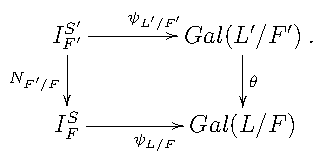
\includegraphics[width=0.2604\paperwidth]{images/L2-p015-diagram.pdf}\end{figure}
\sourcepage{16}
这里$S$是$\OO_F$中包含所有在$L'$中分歧的素理想的任意有限集，$S'$是$\OO_{F'}$中位于$S$中的素理想上方的所有素理想组成的集合。$\theta$是由以下复合给出的自然映射：
\[\Gal(L'/F')\longrightarrow\Gal(LF'/F')\longrightarrow\Gal(LF'/F)\longrightarrow\Gal(L/F).\]
\end{proposition}
\eref{命题}{L2S3O2}的证明直接，留给读者作为练习。
\originalnumber{3}
\begin{corollary}\label{L2S3O3}
Artin映射$\psi_{L/F}$为满射。
\end{corollary}
\begin{proof}
记$G'$为$\psi_{L/F}$的像。由Galois理论，存在中间域$F\subseteq K\subseteq L$，使$\Gal(K/F)=\Gal(L/F)/G'$且$\Gal(L/K)\cong G'$。因此，由\eref{命题}{L2S3O2}和\eref{笔记}{L2S3O1}，$F$中除有限多个以外的所有素理想都在$K$中完全分裂。由下面的命题，$K=F$。
\end{proof}
\originalnumber{4}
\begin{proposition}\label{L2S3O4}
设$K/F$为代数数域的有限扩张。如果$F$中除有限多个以外的所有素理想都在$K$中完全分裂，则$F=K$。（\bref{L2refN6}{N}第VI章第3节推论3.8。）
\end{proposition}
\originalnumber{5}
\begin{corollary}\label{L2S3O5}
$N_{L/F}(I_L^S)$包含于$\psi_{L/F}$的核。
\end{corollary}
\begin{proof}
在\eref{命题}{L2S3O2}中取$L'=L=F'$即可。
\end{proof}
回忆，$F$的无穷素位就是$F$的阿基米德素位，它与共轭嵌入对$(\iota,\overline\iota:F\hookrightarrow\C)$一一对应。若一个无穷素位$\infty$对应于$\iota_\infty=\overline\iota_\infty:F\hookrightarrow\R$，则称它为实素位；否则称为复素位。\znote{素位（place）是域上绝对值的等价类，等价指诱导同一拓扑。对代数数域 $F$，非阿基米德素位一一对应 $\OO_F$ 的非零素理想，阿基米德素位一一对应 $F\hookrightarrow\C$ 的嵌入的共轭类：实嵌入给出实素位，共轭嵌入对给出复素位。引进素位是为了让分歧、范数与 $L$ 函数在有限处与无穷处获得统一表述。[来源：nLab "place"，\url{https://ncatlab.org/nlab/show/place}（Last revised 2015-12-17；2026-11-14 访问）。]}\idx{无穷素位}

Artin互反律把$\ker\psi_{L/F}$描述为一个模$\mathfrak{m}$的同余子群。首先，定义$F$的一个\textbf{模}为形式乘积\idx{模（类域论）}
\[\mathfrak{m}=\prod_{\p}\p^{n(\p)},\]
其中$\p$遍历$F$的所有素位（包括无穷素位）。指数$n(\p)$为非负整数，只有有限多个为正；此外，若$\infty$为实素位，$n(\infty)$只能是$0$或$1$；若为复素位，则$n(\infty)=0$。
\sourcepage{17}
若$n(\p)>0$，就说素位$\p$整除$\mathfrak{m}$。记$I_F^{\mathfrak{m}}=I_F^S$，其中$S$为所有整除$\mathfrak{m}$的有限素位组成的集合。\par\needspace{5\baselineskip}定义
\[
F_{\mathfrak{m},1}=\left\{0\ne a\in F\ \middle|\ \begin{array}{l}\ord_{\p}(a-1)\geq n(\p)\text{，对所有有限素位 }\p\mid\mathfrak{m},\\\iota_\infty(a)>0\text{，对所有 }\infty\mid\mathfrak{m}\end{array}\right\}.
\]
$F_{\mathfrak{m},1}$的每个元素都给出一个$F$的主分式理想，因此有映射$i:F_{\mathfrak{m},1}\longrightarrow I_F$，其像包含于$I_F^{\mathfrak{m}}$。商群
\[C_{\mathfrak{m}}:=I_F^{\mathfrak{m}}/i(F_{\mathfrak{m},1})\]
称为\textbf{模$\mathfrak{m}$的射线类群}\znote{射线类群是理想类群的同余推广：$C_{\mathfrak{m}}=I_F^{\mathfrak{m}}/i(F_{\mathfrak{m},1})$ 把主理想换成由满足 $a\equiv1\pmod{\mathfrak{m}}$（在实素位处还要求 $a>0$）的元素生成的主理想。$\mathfrak{m}=1$ 时它退回通常的理想类群；模越大，$C_{\mathfrak{m}}$ 越大，而它恰参数化模 $\mathfrak{m}$ 的射线类域。注意 $i(F_{\mathfrak{m},1})$ 由主理想构成，故 $C_{\mathfrak{m}}$ 仍是「理想模主理想」型的商群，只是分子分母都加上了同余限制。[来源：Neukirch, \textit{Algebraic Number Theory}, Grundlehren der mathematischen Wissenschaften 322, 第 VI 章（本讲参考文献）。]}\idx{射线类群}
\originalnumber{6}
\begin{note}[L2S3O6]
若$\mathfrak{m}=1$，即所有指数$n(\p)$都为零，则$C_{\mathfrak{m}}$就是$F$的通常的类群，即分式理想群对主理想群取商所得的群。
\end{note}
\originalnumber{7}
\begin{theorem}{互反律}\label{L2S3O7}\idx{Artin互反律}
设$L$为$F$的有限阿贝尔扩张。则存在一个被所有在$L$中分歧的素理想整除的模$\mathfrak{m}$，使
\[\ker\psi_{L/F}=N_{L/F}(I_L^{\mathfrak{m}})\,i(F_{\mathfrak{m},1}).\]
换言之，$\Gal(L/F)\cong I_F^{\mathfrak{m}}/\bigl(N_{L/F}(I_L^{\mathfrak{m}})\,i(F_{\mathfrak{m},1})\bigr)$。
\end{theorem}
\originalnumber{8}
\begin{note}[L2S3O8]
Artin互反律有时写成表面上不同的形式，例如使用解析性质来表述，但它们本质上相同。
\end{note}
\originalnumber{9}
\begin{theorem}{存在唯一性定理}\label{L2S3O9}\idx{射线类域}
对$F$的任意模$\mathfrak{m}$，存在一个在同构意义下唯一的域$L_{\mathfrak{m}}$，称为\textbf{模$\mathfrak{m}$的射线类域}，使Artin映射定义同构$C_{\mathfrak{m}}\longrightarrow\Gal(L_{\mathfrak{m}}/F)$。
\end{theorem}
注意，$C_{\mathfrak{m}}$为阿贝尔群，故$L_{\mathfrak{m}}/F$是阿贝尔扩张。
\originalnumber{10}
\begin{corollary}{分类定理}\label{L2S3O10}
\begin{enumerate}
\item 设$H$为模$\mathfrak{m}$的同余子群，即$i(F_{\mathfrak{m},1})\subseteq H\subseteq I_F^{\mathfrak{m}}$。则存在阿贝尔扩张$L/F$，使$H=N_{L/F}(I_L^{\mathfrak{m}})\,i(F_{\mathfrak{m},1})$。
\item 每个有限阿贝尔扩张$L/F$都是某个射线类域的子扩张。
\end{enumerate}
\end{corollary}
现在可以把Kronecker--Weber定理作为\eref{推论}{L2S3O10}的特例来证明。
% [Tutor Note: 原书 p17 末作 "as a special case to Corollary 3.5"，按上下文应为推论 3.10（分类定理）；译文按正确编号处理。]
\sourcepage{18}
\begin{proof}[Kronecker--Weber定理的证明]
只需证明：对$\Q$的任意模$\mathfrak{m}$，模$\mathfrak{m}$的射线类域是某个分圆域的子扩张。注意，$\Q$只有一个无穷素位，记为$\infty$。若$\mathfrak{m}=m=p_1^{n_1}\cdots p_t^{n_t}$为正整数，则
\[I_{\Q}^{\mathfrak{m}}=\{(a/b)\mid(a,m)=(b,m)=1\},\]
\[\Q_{\mathfrak{m},1}=\{a/b\mid a,b\in\Z,\ a\equiv b\pmod m,\ (a,m)=1\},\]
并且
\[I_{\Q}^{\mathfrak{m}}\supseteq i(\Q_{\mathfrak{m},1})=\{(a/b)\mid a,b\in\Z_{>0},\ a\equiv\pm b\pmod m,\ (a,m)=1\}.\]
考察Artin映射$\psi_{\Q(\zeta_m)/\Q}:I_{\Q}^{\mathfrak{m}}\longrightarrow(\Z/m\Z)^\times$。对任意$p\nmid m$，由\eref{例题}{L2S1O1}，$\operatorname{Fr}[(p)]=[p]\in(\Z/m\Z)^\times$。因此
\[\ker\psi_{\Q(\zeta_m)/\Q}=\{(a/b)\mid a,b>0,\ (a,m)=(b,m)=1,\ a\equiv b\pmod m\}.\]
于是$\ker\psi_{\Q(\zeta_m)/\Q}\subseteq i(\Q_{\mathfrak{m},1})$，故模$\mathfrak{m}$的射线类域是$\Q(\zeta_m)$的子扩张，具体就是$\Q(\zeta_m+\zeta_m^{-1})$。

容易看出，$\Q(\zeta_m)$本身是模$\mathfrak{m}=m\cdot\infty$的射线类域。
\end{proof}
\needspace{5\baselineskip}\section{第2讲参考文献}\label{L2S4}
\needspace{4\baselineskip}关于Dedekind整环的扩张及Hilbert分歧理论：
\begin{references}\refitem{L2refN1}{N} J. Neukirch, \textit{Algebraic number theory}, Grundlehren der mathematischen Wissenschaften 322, Springer-Verlag Berlin Heidelberg GmbH, Chapter I \S8,\S9.\end{references}
\needspace{4\baselineskip}关于分圆域中的分歧：
\begin{references}\refitem{L2refIM}{IM} Kenneth Ireland and Michael Rosen, \textit{A Classical Introduction to Modern Number Theory}, Springer-Verlag New York, Inc. in 1990, Chapter 13 \S2.\end{references}
\needspace{4\baselineskip}关于整体类域论：
\begin{references}
\refitem{L2refN6}{N} J. Neukirch, \textit{Algebraic number theory}, Grundlehren der mathematischen Wissenschaften 322, Springer-Verlag Berlin Heidelberg GmbH, Chapter VI.
\refitem{L2refCF}{CF} J. W. S. Cassels and A. Fr\"ohlich, \textit{Algebraic Number Theory}, Proceedings of an instructional conference organized by the LMS, Chapter VII.
\end{references}
